% $Id: Attitude.tex,v 1.1 2008/01/31 18:04:16 dconway Exp $
\chapter{\label{chapter:Attitude}Attitude}
\chapauthor{Wendy C. Shoan}{Goddard Space Flight Center}

\section{Introduction}

GMAT provides the capability to model the attitude of a spacecraft.  The attitude can be computed in any of three different ways: kinematically, by performing six-degree-of-freedom calculations, or by reading an attitude file (format(s) TBD).  The current version of GMAT has only two types of kinematic modeling available; other methods are to be implemented at a later date.

\section{Design Overview}

When the user creates a Spacecraft object, via the GUI or a script, and s/he needs to compute or report the attitude of that spacecraft at one or more times during the run, s/he must specify a type of attitude for the spacecraft.  The user must also set initial data on the spacecraft attitude.

A Spacecraft object therefore contains a pointer to one Attitude object, of the type specified by the user.  This object will need to be created and set for the spacecraft using its SetRefObject method.  The spacecraft object contains a method to return its attitude as a direction cosine matrix, and a method to return its angular velocity.

GMAT can model several different types of attitude, as mentioned above, each computing the attitude differently.  However, since the types of attitude representations are common to all models, many of the data and methods for handling attitude are contained in a base class, from which all other classes derive.

The base class for all attitude components is the Attitude class.  It contains data and methods required to retrieve spacecraft attitude and attitude rate data.  The method that computes the attitude is included as a pure virtual method, and must be implemented in all leaf classes.

The base Attitude class contains methods that allow the user, the spacecraft, or other GMAT subsystems, to request attitude and attitude rate data in any of several different parameterizations.  Attitude may be returned as a quaternion, a direction cosine matrix, or a set of Euler angles and a sequence.  An attitude rate is retrievable as an angular velocity or as an Euler axis and angle (computed using the Euler sequence).

Also included in the base Attitude class are many static conversion methods, allowing other parts of GMAT to convert one attitude (or attitude rate) parameterization to another, depending on its needs, without having to reference a specific spacecraft or attitude object.

As mentioned above, GMAT includes several different attitude models.  Kinematic attitude propagation options are 1) a Coordinate System Fixed (CSFixed) attitude; 2) a Spinner attitude; and 3) Three-Axis Stabilized attitude (TBD).

To implement these, GMAT currently has a Kinematic class that is derived from the Attitude class.  The CSFixed (Coordinate System Fixed) and Spinner attitude classes derive from the Kinematic class and, as leaf classes, contain implementations of the method, inherited from the base class Attitude, that computes the attitude at the requested time.

\section{Class Hierarchy Summary}

\begin{figure}
\begin{center}
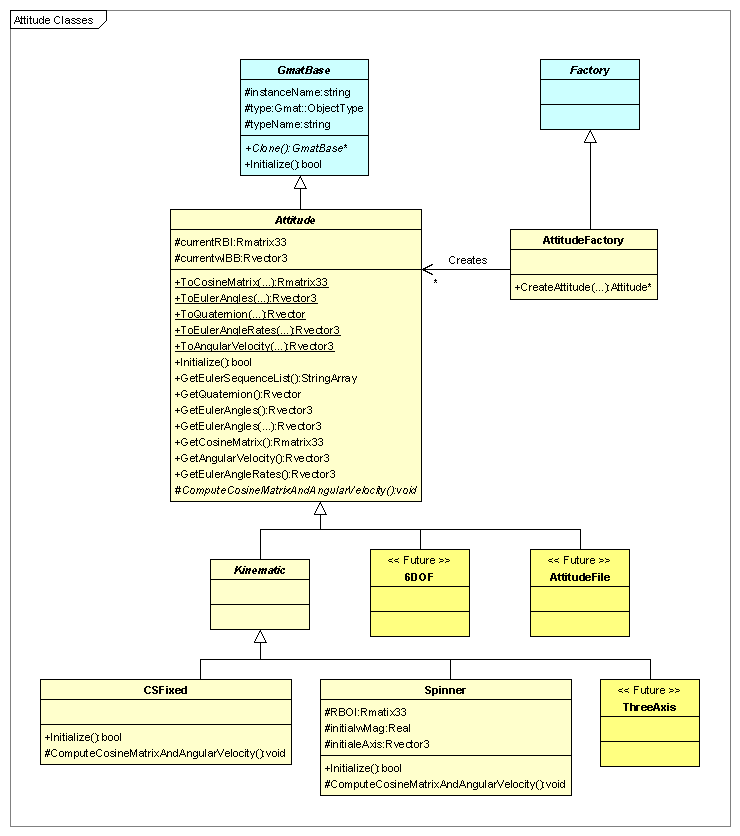
\includegraphics[430,485]{Images/AttitudeClasses.png}
\caption{\label{figure:AttitudeClasses}Attitude Classes}
\end{center}
\end{figure}

This section describes the current attitude classes in GMAT, summarizing key features and providing additional information about the class members.  Figure~\ref{figure:AttitudeClasses} presents the class diagram for this subsystem.

\subsubsection{Attitude}

The Attitude class is the base class for all attitude classes.  Any type of attitude that is created by user specification, via a script or the GUI, will therefore include all public or protected data members and methods contained in the Attitude class.  Key data and methods are:

\subparagraph{\textit{Data members}}

\begin{itemize}
\item \textbf{eulerSequenceList}:  a list of strings representing all of the possible Euler sequences that may be selected by the user
\item \textbf{refCSName}: the name of the reference coordinate system - the user must supply this
\item \textbf{refCS}: a pointer to the reference coordinate system - this must be set using the attitude object's SetRefObject method
\item \textbf{initialEulerSeq}: an UnsignedIntArray containing the three values of the initial Euler sequence
\item \textbf{initialEulerAng}: an Rvector3 containing the three initial Euler angles (degrees)
\item \textbf{initialDcm}: an Rmatrix33 containing the initial direction cosine matrix
\item \textbf{initialQuaternion}: Rvector representation of the initial quaternion
\item \textbf{initialEulerAngRates}: Rvector3 containing the initial Euler angle rates (degrees/second)
\item \textbf{initialAngVel}: Rvector3 containing the initial angular velocity (degrees/second)
\end{itemize}

\subparagraph{\textit{Methods}}

\begin{itemize}
\item \textbf{GetEpoch()}: returns the epoch for the attitude
\item \textbf{SetEpoch(Real toEpoch)}: sets the value for the attitude; this method is called by the GUI, script interpreter or spacecraft
\item \textbf{SetReferenceCoordinateSystemName(const std::string \&refName)}: sets the reference coordinate system name
\item \textbf{GetEulerSequenceList()}: returns a list of strings representing all possible Euler sequence values
\item \textbf{GetQuaternion(Real atTime)}: returns the quaternion representation of the attitude, computed at the A1Mjd time atTime
\item \textbf{GetEulerAngles(Real atTime)}: returns the Euler angle representation of the attitude, computed at the A1Mjd time atTime
\item \textbf{GetCosineMatrix(Real atTime)}: returns the direction cosine matrix representation of the attitude, computed at the A1Mjd time atTime
\item \textbf{GetAngularVelocity(Real atTime)}: returns the angular velocity representation of the attitude rate, computed at the A1Mjd time atTime
\item \textbf{GetEulerAngleRates(Real atTime)}: returns the Euler angle rates representation of the attitude rate, computed at the A1Mjd time atTime
\end{itemize}

In addition to class methods, there are several static methods in the base Attitude class that may be used without instantiating an object of type Attitude.  These are all methods to convert between attitude representations or between attitude rate representations (angles are assumed to be in radians).  They are:

\begin{itemize}
\item \textbf{ToCosineMatrix(const Rvector \&quat1)}: converts the input quaternion to a direction cosine matrix
\item \textbf{ToCosineMatrix(const Rvector3 \&eulerAngles, Integer seq1, Integer seq2, Integer seq3)}: converts the input Euler angles and sequence to a direction cosine matrix
\item \textbf{ToEulerAngles(const Rvector \&quat1, Integer seq1, Integer seq2, Integer seq3)}: converts the input quaternion to Euler angles, given the input Euler sequence
\item \textbf{ToEulerAngles(const Rmatrix33 \&cosMat, Integer seq1, Integer seq2, Integer seq3)}: converts the input direction cosine matrix to Euler angles, given the input Euler sequence
\item \textbf{ToQuaternion(const Rvector3 \&eulerAngles, Integer seq1, Integer seq2, Integer seq3)}: converts the input set of Euler angles and sequence to a quaternion
\item \textbf{ToQuaternion(const Rmatrix33 \&cosMat)}: converts the input direction cosine matrix to a quaternion
\item \textbf{ToEulerAngleRates(const Rvector3 angularVel, Integer seq1, Integer seq2, Integer seq3)}: converts the input angular velocity to Euler angle rates, using the input Euler sequence
\item \textbf{ToEulerAngleRates(const Rvector3 eulerRates, Integer seq1, Integer seq2, Integer seq3)}: converts the input Euler angle rates to angular velocity, using the input Euler sequence
\end{itemize}

\subsubsection{Kinematic}

The Kinematic class is the base class for the kinematic models: Coordinate System Fixed, Spinner, and Three-Axis Stablized (TBD).  At this time, there are no additional data members or methods for this class.

\subsubsection{CSFixed}

The CSFixed class models a Coordinate System Fixed attitude.  The user supplies the initial attitude and specifies the reference coordinate system, from the current set of default and user-defined coordinate systems, to which the attitude is fixed.  Since the attitude is fixed to this coordinate system, no initial attitude rate need be provided.  The code in this class then computes the attitude at a requested time using the initial input data and the rotation matrix between the reference coordinate system and the inertial coordinate system at the specified time, obtained from the Coordinate System subsystem.  There are no significant data members.

\subparagraph{\textit{Methods}}

\begin{itemize}
\item \textbf{ComputeCosineMatrixAndAngularVelocity(Real atTime)}: computes the direction cosine matrix and angular velocity at the requested time; these data can then be retrieved in other representations as well
\end{itemize}

\subsubsection{Spinner}

This class models a Spinner attitude.  The user must supply an initial attitude and reference coordinate system when initializing a Spinner attitude.  In addition, s/he must provide an initial attitude rate.  This rate does not change over time, for this model.  The initial epoch is expected to be an A1Mjd time, input as a Real, and is assumed to be the same as the orbit epoch (i.e. when the orbit epoch is set, the spacecraft knows to use that epoch for the attitude as well).  This class can then compute the attitude at a specified time, using the initial input data and the rotation matrix from the reference coordinate system to the inertial coordinate system at the epoch time.  It contains some protected data members to store data computed on initialization.

\subparagraph{\textit{Methods}}

\begin{itemize}
\item \textbf{ComputeCosineMatrixAndAngularVelocity(Real atTime)}: computes the direction cosine matrix and angular velocity at the requested time; these data can then be retrieved in other representations as well
\end{itemize}

\section{Program Flow}

After an Attitude object is created and passed to a Spacecraft object, the initial data must be set.  Then, as it is for most objects, the Initialize method must be called on the attitude.  After that, the Attitude object is ready to compute the spacecraft attitude at any time requested.

\subsection{Initialization}

As mentioned above, the user must specify attitude initial data for a spacecraft, via the GUI or the script.  An example script appears here:

\begin{quote}
\begin{verbatim}
%------------------------------------------------------------------------
%------------------ Spacecraft Attitude Mode ----------------------------
%------------------------------------------------------------------------
Sat.AttitudeMode = {Kinematic, 6DOF, FromFile};
Sat.KinematicAttitudeType = { Spinner, CSFixed};  % 3-Axis TBD

%------------------------------------------------------------------------
%------------------ Spacecraft Attitude Coordinate System ---------------
%------------------------------------------------------------------------
Sat.AttitudeCoordinateSystem = MJ2000Ec;

%------------------------------------------------------------------------
%-------------- Spacecraft Attitude Initial Data ------------------------
%------------------------------------------------------------------------
Sat.AttitudeStateType = {EulerAngles, Quaternion, DCM};
Sat.EulerAngleSequence = {123, 132, 213, 312, ... 321};
Sat.EulerAngle1 = 5.0;    % degrees
Sat.EulerAngle2 = 10.0;    % degrees
Sat.EulerAngle3 = 15.0;    % degrees
% Sat.q1 = 0.0;   % these are set if the type is Quaternion
% Sat.q2 = 0.0;
% Sat.q3 = 0.0;
% Sat.q4 = 1.0;
% Sat.DCM11 = 1.0;     % set if attitude type is DCM
% Sat.DCM12 = 0.0;
...
% Sat.DCM33 = 1.0;

Sat.AttitudeRateStateType = {EulerAngleRates, AngularVelocity};
Sat.EulerAngleRate1 = 5.0;
Sat.EulerAngleRate2 = 5.0;
Sat.EulerAngleRate3 = 5.0;
% Sat.AngularVelocityX = 5.0;  % set if attitude rate type is angular velocity
% Sat.AngularVelocityY = 5.0;
% Sat.AngularVelocityZ = 5.0;
\end{verbatim}
\end{quote}

In all models, the initial attitude may be input as a direction cosine matrix, a quaternion, or a set of Euler angles and sequence.  The initial rate may be input as an angular velocity or as an Euler axis and angle (to be used along with an Euler sequence from the input attitude specification).

\subsection{Computation}

GMAT uses the initial data to compute the attitude at any time requested.  For better performance, GMAT keeps track of the last attitude computed, and the time for which it was computed, and only recomputes when necessary.

For the two models implemented thus far, it is necessary for GMAT to compute a rotation matrix (and for the CSFixed attitude, its derivative as well) between the inertial (MJ2000 Equatorial) coordinate system and the specified reference coordinate system.  GMAT has this capability, implemented in its Coordinate System subsystem.

